% !TeX root = RJwrapper.tex
\title{Kfre: An R Package for Kidney Failure Risk Estimation Using the Kidney Failure Risk Equation}


\author{by Leonid Shpaner}

\maketitle

\abstract{%
Chronic kidney disease (CKD) affects hundreds of millions of people worldwide, and identifying patients at highest risk of progression to kidney failure is critical for timely clinical intervention. The Kidney Failure Risk Equation (KFRE), developed by Tangri and colleagues and validated across more than 700,000 individuals in 30 countries, provides 2- and 5-year probability estimates of kidney failure using 4, 6, or 8 clinical variables. Despite its widespread clinical adoption and endorsement by KDIGO guidelines, no dedicated, feature-complete R implementation existed prior to this work. The kfre package fills this gap by providing vectorized KFRE predictions across all three model variants and both time horizons, a convenience wrapper for appending risk columns to data frames, CKD stage and ESRD outcome classification utilities, urine protein-to-creatinine ratio conversion, and publication-ready ROC and precision-recall curve plotting. The package is designed with three complementary interfaces: a functional API, a data-frame wrapper, and an R6 class, to serve clinicians, analysts, and pipeline developers alike. This paper describes the package design, implementation, and a fully reproducible demonstration using synthetic patient data. This package is available from the Comprehensive R Archive Network at \url{https://CRAN.R-project.org/package=kfre}
}

\section{Introduction}\label{introduction}

Chronic kidney disease (CKD) is a major global health burden, affecting an
estimated 10-15\% of adults worldwide \citep{bikbov2020global}. For the subset of
patients whose disease progresses to kidney failure, requiring dialysis or
transplantation, the clinical and economic consequences are severe.
Identifying these high-risk individuals early enough to intervene meaningfully
is one of the central challenges of nephrology practice.

The Kidney Failure Risk Equation (KFRE) was developed by \citet{tangri2011} using data
from two Canadian cohorts of patients with CKD stages G3-G5, and subsequently
validated by \citet{tangri2016} in over 700,000 individuals spanning more than 30
countries. The KFRE provides individualized 2- and 5-year probability estimates
of progression to kidney failure using either four variables (age, sex, estimated
glomerular filtration rate {[}eGFR{]}, and urine albumin-to-creatinine ratio
{[}uACR{]}), six variables (adding diabetes and hypertension status), or eight
variables (additionally incorporating serum albumin, phosphorus, bicarbonate,
and calcium). It has since been incorporated into electronic health record
systems, reimbursement criteria, and international clinical practice guidelines.
Specifically, the Kidney Disease: Improving Global Outcomes (KDIGO) 2024
guidelines recommend KFRE as the standard tool for estimating absolute kidney
failure risk in patients with CKD stages G3-G5 \citep{kdigo2024}.

Despite this broad clinical adoption, researchers and data analysts working in R
lacked a dedicated, full-featured package for computing KFRE estimates,
classifying CKD staging, converting protein measurement units, and evaluating
model performance, all within a single, coherent interface. Prior to \textbf{kfre},
analysts typically implemented the equations manually or adapted code from other
languages, introducing opportunities for transcription errors and inconsistencies
across projects. The \textbf{kfre} package \citep{shpaner2025kfre} addresses this gap.

A companion Python implementation exists (available via PyPI), and \textbf{kfre} is
designed to maintain parity with it in naming conventions, output shapes, and
expected column structures, facilitating cross-language reproducibility in
research pipelines that use both R and Python.

The remainder of this paper is organized as follows. We describe the KFRE
methodology in Section 2, the package design and architecture in Section
3, each major component of the API in Section 4, a reproducible worked example
in Section 5, and concluding discussion in Section 6.

\section{Background}\label{background}

\subsection{The KFRE risk model}\label{the-kfre-risk-model}

The KFRE models the probability of kidney failure within a given time horizon
using a proportional hazards framework. For a patient with covariate vector
\(\mathbf{x}\), the predicted probability of kidney failure within \(t\) years is:

\[
P(\text{kidney failure within } t \text{ years} \mid \mathbf{x}) =
1 - S_0(t)^{\exp(\mathbf{x}^T \boldsymbol{\beta} - c)}
\]

where \(S_0(t)\) is the baseline survival probability at horizon \(t\),
\(\boldsymbol{\beta}\) is the vector of published log-hazard coefficients,
and \(c\) is a centering constant equal to the mean linear predictor in the
derivation cohort. The term \(\exp(\mathbf{x}^T \boldsymbol{\beta} - c)\)
is the relative hazard for the individual patient relative to the average
patient in the derivation sample.

The linear predictor for the 4-variable model takes the form:

\[
\eta_4 = \beta_{\text{age}} \cdot \text{age} +
          \beta_{\text{sex}} \cdot \mathbf{1}[\text{male}] +
          \beta_{\text{eGFR}} \cdot \text{eGFR} +
          \beta_{\text{uACR}} \cdot \ln(\text{uACR})
\]

The 6-variable model extends this with:

\[
\eta_6 = \eta_4 +
          \beta_{\text{dm}} \cdot \mathbf{1}[\text{diabetes}] +
          \beta_{\text{htn}} \cdot \mathbf{1}[\text{hypertension}]
\]

And the 8-variable model further adds:

\[
\eta_8 = \eta_6 +
          \beta_{\text{alb}} \cdot \text{albumin} +
          \beta_{\text{phos}} \cdot \text{phosphorus} +
          \beta_{\text{bicarb}} \cdot \text{bicarbonate} +
          \beta_{\text{ca}} \cdot \text{calcium}
\]

Note that uACR enters as its natural logarithm, reflecting the
log-linear relationship between albuminuria and kidney failure risk
observed across the derivation and validation cohorts.

\subsection{Published coefficients}\label{published-coefficients}

Table \ref{tab:coef-table} presents the published coefficients from
\citet{tangri2016} for all three model variants. The coefficients are identical
across the 2-year and 5-year horizons within each population stratum;
only the baseline survival probability \(S_0(t)\) differs by horizon.

\begin{table}

\caption{\label{tab:coef-table}Published KFRE log-hazard coefficients from Tangri et al. (2016) for North American populations.}
\centering
\begin{tabular}[t]{llll}
\toprule
Variable & 4-variable & 6-variable & 8-variable\\
\midrule
Age (per year) & -0.2201 & -0.2201 & -0.1992\\
Sex (male = 1) & -0.2467 & -0.2467 & -0.3580\\
eGFR (per mL/min/1.73 m\textsuperscript{2}) & -0.5567 & -0.5567 & -0.4510\\
ln(uACR) (per unit) & 0.4510 & 0.4510 & 0.3770\\
Diabetes mellitus & --- & 0.2097 & 0.1870\\
\addlinespace
Hypertension & --- & 0.1031 & 0.1430\\
Albumin (g/dL) & --- & --- & -0.3010\\
Phosphorus (mg/dL) & --- & --- & 0.2030\\
Bicarbonate (mEq/L) & --- & --- & -0.1360\\
Calcium (mg/dL) & --- & --- & -0.1830\\
\bottomrule
\end{tabular}
\end{table}

\subsection{Baseline survival probabilities}\label{baseline-survival-probabilities}

The baseline survival probabilities \(S_0(t)\) differ by time horizon and
by whether the North American or non-North American calibration is applied.
Table \ref{tab:s0-table} presents these values as reported by \citet{tangri2016}.
The non-North American values are systematically lower, reflecting higher
observed event rates in international cohorts relative to the Canadian
derivation sample.

\begin{table}

\caption{\label{tab:s0-table}Baseline survival probabilities $S_0(t)$ by model, time horizon, and population.}
\centering
\begin{tabular}[t]{llll}
\toprule
Model & Horizon & North American & Non-North American\\
\midrule
4-variable & 2-year & 0.9832 & 0.9766\\
4-variable & 5-year & 0.9365 & 0.9240\\
6-variable & 2-year & 0.9832 & 0.9766\\
6-variable & 5-year & 0.9365 & 0.9240\\
8-variable & 2-year & 0.9769 & 0.9695\\
\addlinespace
8-variable & 5-year & 0.9240 & 0.9113\\
\bottomrule
\end{tabular}
\end{table}

The non-North American calibration applies a multiplicative shift to the
baseline survival. If \(S_0^{\text{NA}}(t)\) denotes the North American
baseline survival and \(S_0^{\text{non-NA}}(t)\) the international value,
the recalibrated probability for a patient with linear predictor \(\eta\) is
simply:

\[
P^{\text{non-NA}}(t \mid \mathbf{x}) =
1 - \left[S_0^{\text{non-NA}}(t)\right]^{\exp(\eta - c)}
\]

This recalibration adjusts the overall event rate while preserving the
relative ranking of patients by risk, since the coefficient vector
\(\boldsymbol{\beta}\) is held constant across populations.

\subsection{uPCR to uACR conversion}\label{upcr-to-uacr-conversion}

The KFRE requires uACR as input, but many clinical datasets record only
urine protein-to-creatinine ratio (uPCR). \textbf{kfre} implements the
sex-, diabetes-, and hypertension-stratified log-linear regression equations
from \citet{sumida2020}. The general form is:

\[
\ln(\hat{\text{uACR}}) = \alpha_k + \beta_k \cdot \ln(\text{uPCR})
\]

where \(k\) indexes the subgroup defined by sex, diabetes status, and
hypertension status, and \(\alpha_k\), \(\beta_k\) are the subgroup-specific
intercept and slope estimated by \citet{sumida2020} from a large multi-ethnic CKD
cohort. Exponentiating gives the predicted uACR on the original scale:

\[
\hat{\text{uACR}} = \exp\!\left(\alpha_k + \beta_k \cdot \ln(\text{uPCR})\right)
\]

This approach produces better-calibrated uACR estimates than a simple fixed
ratio because the uPCR-to-uACR relationship varies systematically with
patient characteristics: diabetic patients tend to excrete proportionally
more albumin relative to total protein, and females tend to have lower
creatinine excretion, both of which affect the ratio between the two
measurements.

\section{Package design}\label{package-design}

\subsection{Design philosophy}\label{design-philosophy}

\textbf{kfre} is designed around three complementary usage patterns that reflect
distinct user types and workflows in clinical research:

\textbf{Single-person queries} are served by the \texttt{kfre\_person()} function (also
available as a method on the \texttt{RiskPredictor} R6 object). This interface accepts
individual scalar values and is well-suited for interactive exploration,
clinical decision support prototyping, or embedding in Shiny applications.

\textbf{Cohort-level analysis} is served by \texttt{add\_kfre\_risk\_col()}, a convenience
wrapper that accepts a data frame and column name mappings and returns the same
data frame augmented with one new column per requested model-and-horizon
combination. This follows the common R idiom of returning an enriched data
frame and fits naturally into \textbf{dplyr}-style analysis pipelines.

\textbf{Programmatic and pipeline use} is served by the \texttt{RiskPredictor} R6 class,
which encapsulates the data frame and column mappings at construction time and
exposes a \texttt{predict\_kfre()} method for vectorized prediction. This design is
particularly useful for developers building larger clinical data pipelines where
the predictor object is passed between functions or modules, and for users
coming from Python who are familiar with scikit-learn-style fit/predict
patterns.

This multi-interface approach means that a nephrologist testing a single patient,
a biostatistician processing a registry cohort, and a software engineer building
an EHR plugin can all use \textbf{kfre} via the interface most natural to their
context.

\subsection{Dependencies}\label{dependencies}

\textbf{kfre} imports \textbf{R6} \citep{chang2021} for the object-oriented interface,
\textbf{ggplot2} \citep{wickham2016} for plotting, \textbf{pROC} \citep{robin2011} for ROC
curve computation, and \textbf{precrec} \citep{saito2015} for precision-recall curve
computation. The choice of \textbf{pROC} and \textbf{precrec} in preference to
computing metrics manually was deliberate: these packages implement partial AUC,
confidence intervals, and bootstrapping that would otherwise require substantial
additional code, and they maintain parity with the metric implementations in the
companion Python package.

\subsection{Object model}\label{object-model}

The \texttt{RiskPredictor} class uses the R6 object model. The R6 approach was chosen
over S3 or S4 because the class encapsulates both data state (the input data
frame and column mapping) and behavior (the prediction methods) in a way that is
more natural for users constructing a predictor once and calling it multiple
times. This also simplifies the public API by reducing the number of arguments
that must be repeated across multiple calls.

The functional wrappers \texttt{predict\_kfre()} and \texttt{add\_kfre\_risk\_col()} are thin
convenience layers over the same underlying core function \texttt{risk\_pred\_core()},
ensuring that all interfaces share a single implementation and that any bug fix
propagates to all entry points.

\section{Package components}\label{package-components}

\subsection{\texorpdfstring{Core prediction: \texttt{risk\_pred\_core()}}{Core prediction: risk\_pred\_core()}}\label{core-prediction-risk_pred_core}

\texttt{risk\_pred\_core()} is the internal computation engine. It accepts scalar or
vector inputs (age, sex indicator, eGFR, uACR, and optionally the extended
variables), the desired number of model variables (4, 6, or 8), the prediction
horizon (2 or 5 years), and a logical flag for North American vs.~non-North
American coefficients. It returns a numeric vector of predicted probabilities.
Direct use of \texttt{risk\_pred\_core()} is not required by most users; it is called
internally by the higher-level interfaces.

\subsection{\texorpdfstring{Single-person prediction: \texttt{kfre\_person()}}{Single-person prediction: kfre\_person()}}\label{single-person-prediction-kfre_person}

\texttt{kfre\_person()} provides a named-argument interface for computing the KFRE for
a single patient. This function is intended to be readable at a glance:

\begin{verbatim}
# 4-variable KFRE, 2-year horizon, male patient
rp <- RiskPredictor$new(df = toy, columns = cols)

rp$kfre_person(
  age = 55, is_male = TRUE,
  eGFR = 45, uACR = 120,
  is_north_american = TRUE, years = 2
)
\end{verbatim}

The \texttt{is\_male} argument (rather than a string) was chosen to make the binary
nature of the sex input explicit and to avoid ambiguity over string matching
(e.g., \texttt{"M"} vs.~\texttt{"male"} vs.~\texttt{"Male"}). The \texttt{add\_kfre\_risk\_col()} wrapper
accepts a column of character sex labels and handles normalization internally
via \texttt{perform\_conversions()}.

\subsection{\texorpdfstring{Data-frame wrapper: \texttt{add\_kfre\_risk\_col()}}{Data-frame wrapper: add\_kfre\_risk\_col()}}\label{data-frame-wrapper-add_kfre_risk_col}

For cohort analysis, \texttt{add\_kfre\_risk\_col()} accepts a data frame along with
named arguments mapping KFRE variable names to column names in the data frame.
It returns the data frame with additional columns appended, named using the
convention \texttt{kfre\_\{n\}var\_\{t\}year} (e.g., \texttt{kfre\_4var\_2year}). The \texttt{num\_vars} and
\texttt{years} arguments each accept vectors, so all desired combinations can be
computed in a single call:

\begin{verbatim}
toy <- data.frame(
  age         = c(55, 72),
  sex_txt     = c("male", "female"),
  eGFR        = c(45, 28),
  uACR        = c(120, 800),
  dm          = c(1, 0),
  htn         = c(1, 1),
  albumin     = c(4.2, 3.4),
  phosphorous = c(3.3, 4.6),
  bicarbonate = c(24, 22),
  calcium     = c(9.1, 9.8),
  stringsAsFactors = FALSE
)

toy_kfre <- add_kfre_risk_col(
  df              = toy,
  age_col         = "age",
  sex_col         = "sex_txt",
  eGFR_col        = "eGFR",
  uACR_col        = "uACR",
  dm_col          = "dm",
  htn_col         = "htn",
  albumin_col     = "albumin",
  phosphorous_col = "phosphorous",
  bicarbonate_col = "bicarbonate",
  calcium_col     = "calcium",
  num_vars        = c(4, 6, 8),
  years           = c(2, 5),
  is_north_american = TRUE,
  copy            = TRUE
)
\end{verbatim}

Tables \ref{tab:table-4-6var} and \ref{tab:table-8var} show predicted risk
estimates for both patients across the 4- and 6-variable models and the
8-variable model respectively.

\begin{table}

\caption{\label{tab:table-4-6var}KFRE risk estimates: 4- and 6-variable models.}
\centering
\begin{tabular}[t]{rlrrrrrr}
\toprule
Age & Sex & eGFR & uACR & 4v-2yr & 4v-5yr & 6v-2yr & 6v-5yr\\
\midrule
55 & male & 45 & 120 & 0.0125 & 0.0384 & 0.0120 & 0.0369\\
72 & female & 28 & 800 & 0.1000 & 0.2803 & 0.1094 & 0.3036\\
\bottomrule
\end{tabular}
\end{table}

\begin{table}

\caption{\label{tab:table-8var}KFRE risk estimates: 8-variable model.}
\centering
\begin{tabular}[t]{rlrr}
\toprule
Age & Sex & 8v-2yr & 8v-5yr\\
\midrule
55 & male & 0.0113 & 0.0362\\
72 & female & 0.1193 & 0.3389\\
\bottomrule
\end{tabular}
\end{table}

The \texttt{copy\ =\ TRUE} argument returns a new data frame rather than modifying the
input in place, consistent with R's functional programming conventions and
predictable behavior in pipeline contexts.

\subsection{\texorpdfstring{R6 interface: \texttt{RiskPredictor}}{R6 interface: RiskPredictor}}\label{r6-interface-riskpredictor}

The \texttt{RiskPredictor} R6 class encapsulates a data frame and its column mappings
at construction time, exposing \texttt{predict\_kfre()} for vectorized batch prediction
and \texttt{kfre\_person()} for single-patient queries. This interface is particularly
useful when predictions across multiple model configurations are needed
repeatedly on the same dataset, as the data frame and column map need only be
specified once:

\begin{verbatim}
cols <- list(
  age = "age", sex = "sex_txt", eGFR = "eGFR", uACR = "uACR",
  dm = "dm", htn = "htn", albumin = "albumin",
  phosphorous = "phosphorous", bicarbonate = "bicarbonate",
  calcium = "calcium"
)

rp    <- RiskPredictor$new(df = toy, columns = cols)
p4_2y <- rp$predict_kfre(years = 2, is_north_american = TRUE,
                          use_extra_vars = FALSE, num_vars = 4)
p6_5y <- rp$predict_kfre(years = 5, is_north_american = TRUE,
                          use_extra_vars = TRUE,  num_vars = 6)
p8_2y <- rp$predict_kfre(years = 2, is_north_american = TRUE,
                          use_extra_vars = TRUE,  num_vars = 8)
\end{verbatim}

\begin{table}

\caption{\label{tab:r6-table}Predictions via RiskPredictor R6 interface.}
\centering
\begin{tabular}[t]{lrrr}
\toprule
Patient & 4v-2yr & 6v-5yr & 8v-2yr\\
\midrule
Patient 1 (M, 55) & 0.0125 & 0.0369 & 0.0113\\
Patient 2 (F, 72) & 0.1000 & 0.3036 & 0.1193\\
\bottomrule
\end{tabular}
\end{table}

\subsection{CKD staging and ESRD outcome classification}\label{ckd-staging-and-esrd-outcome-classification}

\texttt{class\_ckd\_stages()} assigns standard CKD stage labels (G1-G5, with G3 split
into G3a and G3b) based on eGFR, following KDIGO classification thresholds.
An optional \texttt{combined\_stage\_col} merges adjacent stages for analyses that use
broader groupings (e.g., G3a/G3b combined as G3).

\texttt{class\_esrd\_outcome()} constructs binary outcome columns from a continuous
follow-up duration and an ESRD event flag, for use as ground-truth labels in
model evaluation. It accepts follow-up time in days (converting internally to
years) and a threshold horizon, returning a binary column indicating whether
the ESRD event occurred within the specified window:

\begin{verbatim}
out <- data.frame(
  eGFR          = c(65, 48, 25, 12),
  ESRD_flag     = c(0, 1, 1, 1),
  followup_days = c(400, 600, 500, 800)
)

out <- class_ckd_stages(
  df = out, egfr_col = "eGFR",
  stage_col = "stage", combined_stage_col = "stage_combined"
)

out <- class_esrd_outcome(
  df = out, col = "ESRD_flag", years = 2,
  duration_col = "followup_days", prefix = "esrd",
  create_years_col = TRUE
)
\end{verbatim}

Applied to four synthetic patients with eGFR values of 65, 48, 25, and
12 mL/min/1.73 m\(^2\), \texttt{class\_ckd\_stages()} assigns stages G2, G3a, G4, and G5
respectively. \texttt{class\_esrd\_outcome()} then labels the 2-year binary outcome:
patients with eGFR 48 and 25 (follow-up of 600 and 500 days, both under 2 years)
are flagged as events, while the patient with eGFR 65 (follow-up 400 days, no
ESRD flag) and the patient with eGFR 12 (follow-up 800 days, exceeding the
2-year window) are labeled 0.

\subsection{\texorpdfstring{uPCR to uACR conversion: \texttt{upcr\_uacr()}}{uPCR to uACR conversion: upcr\_uacr()}}\label{upcr-to-uacr-conversion-upcr_uacr}

The KFRE requires uACR, but many datasets record urine protein-to-creatinine
ratio (uPCR). \textbf{kfre} implements the sex-, diabetes-, and
hypertension-stratified conversion equations from \citet{sumida2020}, which provide
better calibration for clinical populations than a simple fixed ratio:

\begin{verbatim}
df_upcr <- data.frame(
  sex  = c("female", "male", "female"),
  dm   = c(1, 0, 1),
  htn  = c(1, 1, 0),
  upcr = c(150, 600, 50)
)

uacr <- upcr_uacr(
  df_upcr,
  sex_col          = "sex",
  diabetes_col     = "dm",
  hypertension_col = "htn",
  upcr_col         = "upcr",
  female_str       = "female"
)
\end{verbatim}

The three input uPCR values (150, 600, and 50 mg/g) convert to estimated uACR
values of 33.5, 269.06, and
5.29 mg/g respectively, reflecting the sex-, diabetes-, and
hypertension-stratified adjustments applied by the \citet{sumida2020} regression
equations.

\subsection{\texorpdfstring{Model evaluation: \texttt{eval\_kfre\_metrics()}}{Model evaluation: eval\_kfre\_metrics()}}\label{model-evaluation-eval_kfre_metrics}

\texttt{eval\_kfre\_metrics()} computes a suite of performance metrics for each
requested model variant and time horizon. Three metrics are implemented.

The \textbf{Brier score} measures mean squared error between predicted probabilities
\(\hat{p}_i\) and binary outcomes \(y_i \in \{0, 1\}\) over \(n\) patients:

\[
\text{BS} = \frac{1}{n} \sum_{i=1}^{n} (\hat{p}_i - y_i)^2
\]

A Brier score of 0 indicates perfect calibration; a score of 0.25 corresponds
to the performance of an uninformative model that predicts \(\hat{p}_i = 0.5\)
for all patients.

The \textbf{area under the ROC curve} (AUC-ROC) measures the probability that a
randomly chosen event patient receives a higher predicted risk than a randomly
chosen non-event patient:

\[
\text{AUC} = P(\hat{p}_i > \hat{p}_j \mid y_i = 1,\; y_j = 0)
\]

An AUC of 0.5 corresponds to random discrimination; an AUC of 1.0 to perfect
separation of events from non-events.

The \textbf{average precision} (AP) summarizes the precision-recall curve as the
weighted mean of precisions at each threshold, with the increase in recall
from the previous threshold used as the weight:

\[
\text{AP} = \sum_{k} (R_k - R_{k-1}) \cdot P_k
\]

where \(P_k\) and \(R_k\) are the precision and recall at the \(k\)-th threshold.
Average precision is particularly informative for imbalanced datasets where
kidney failure events are rare relative to the total cohort, as it penalizes
models that achieve high recall only at the cost of many false positives.

\texttt{eval\_kfre\_metrics()} expects outcome columns following the naming convention
of \texttt{class\_esrd\_outcome()} (e.g., \texttt{esrd\_2\_year\_outcome}) and prediction columns
following that of \texttt{add\_kfre\_risk\_col()} (e.g., \texttt{kfre\_4var\_2year}). This
convention is enforced consistently so that evaluation requires no additional
column renaming.

\subsection{\texorpdfstring{Visualization: \texttt{plot\_kfre\_metrics()}}{Visualization: plot\_kfre\_metrics()}}\label{visualization-plot_kfre_metrics}

\texttt{plot\_kfre\_metrics()} produces publication-quality ROC and precision-recall
curves using \textbf{ggplot2}. It supports overlaying multiple model variants on
the same axes (useful for comparing the 4-, 6-, and 8-variable models), and can
optionally save plots to disk in PNG or SVG format. The \texttt{plot\_type} argument
accepts \texttt{"auc\_roc"}, \texttt{"pr\_curve"}, or \texttt{"all\_plots"}, and \texttt{mode} controls
whether to compute metrics, plot from pre-computed results, or do both.

\section{Worked example}\label{worked-example}

To demonstrate the full package workflow end to end, we construct a synthetic
dataset of 200 patients with CKD, compute KFRE predictions, assign CKD stages
and ESRD outcome labels, and visualize the distribution of predicted risk
across CKD stages.

\subsection{Synthetic data}\label{synthetic-data}

\begin{verbatim}
set.seed(42)
n <- 200

synth <- data.frame(
  age         = round(runif(n, 40, 85)),
  sex_txt     = sample(c("male", "female"), n, replace = TRUE),
  eGFR        = round(runif(n, 10, 59)),
  uACR        = round(runif(n, 30, 3000)),
  dm          = sample(0:1, n, replace = TRUE, prob = c(0.4, 0.6)),
  htn         = sample(0:1, n, replace = TRUE, prob = c(0.25, 0.75)),
  albumin     = round(runif(n, 2.5, 5.0), 1),
  phosphorous = round(runif(n, 2.5, 6.5), 1),
  bicarbonate = round(runif(n, 18, 28)),
  calcium     = round(runif(n, 8.0, 10.5), 1),
  ESRD_flag   = sample(0:1, n, replace = TRUE, prob = c(0.6, 0.4)),
  followup_days = round(runif(n, 180, 1825)),
  stringsAsFactors = FALSE
)
\end{verbatim}

\subsection{Computing KFRE and staging}\label{computing-kfre-and-staging}

\begin{verbatim}
synth_kfre <- add_kfre_risk_col(
  df = synth, age_col = "age", sex_col = "sex_txt",
  eGFR_col = "eGFR", uACR_col = "uACR",
  dm_col = "dm", htn_col = "htn",
  albumin_col = "albumin", phosphorous_col = "phosphorous",
  bicarbonate_col = "bicarbonate", calcium_col = "calcium",
  num_vars = c(4, 6, 8), years = c(2, 5),
  is_north_american = TRUE, copy = TRUE
)

synth_kfre <- class_ckd_stages(
  df = synth_kfre, egfr_col = "eGFR",
  stage_col = "stage", combined_stage_col = "stage_combined"
)

synth_kfre <- class_esrd_outcome(
  df = synth_kfre, col = "ESRD_flag", years = 2,
  duration_col = "followup_days", prefix = "esrd",
  create_years_col = TRUE
)

synth_kfre <- class_esrd_outcome(
  df = synth_kfre, col = "ESRD_flag", years = 5,
  duration_col = "followup_days", prefix = "esrd",
  create_years_col = FALSE
)
\end{verbatim}

\subsection{Risk distribution by CKD stage}\label{risk-distribution-by-ckd-stage}

The distribution of 4-variable, 2-year KFRE estimates by CKD stage confirms
the expected relationship: patients in more advanced stages carry substantially
higher predicted risk (Figure \ref{fig:risk-by-stage}).

\begin{figure}

{\centering 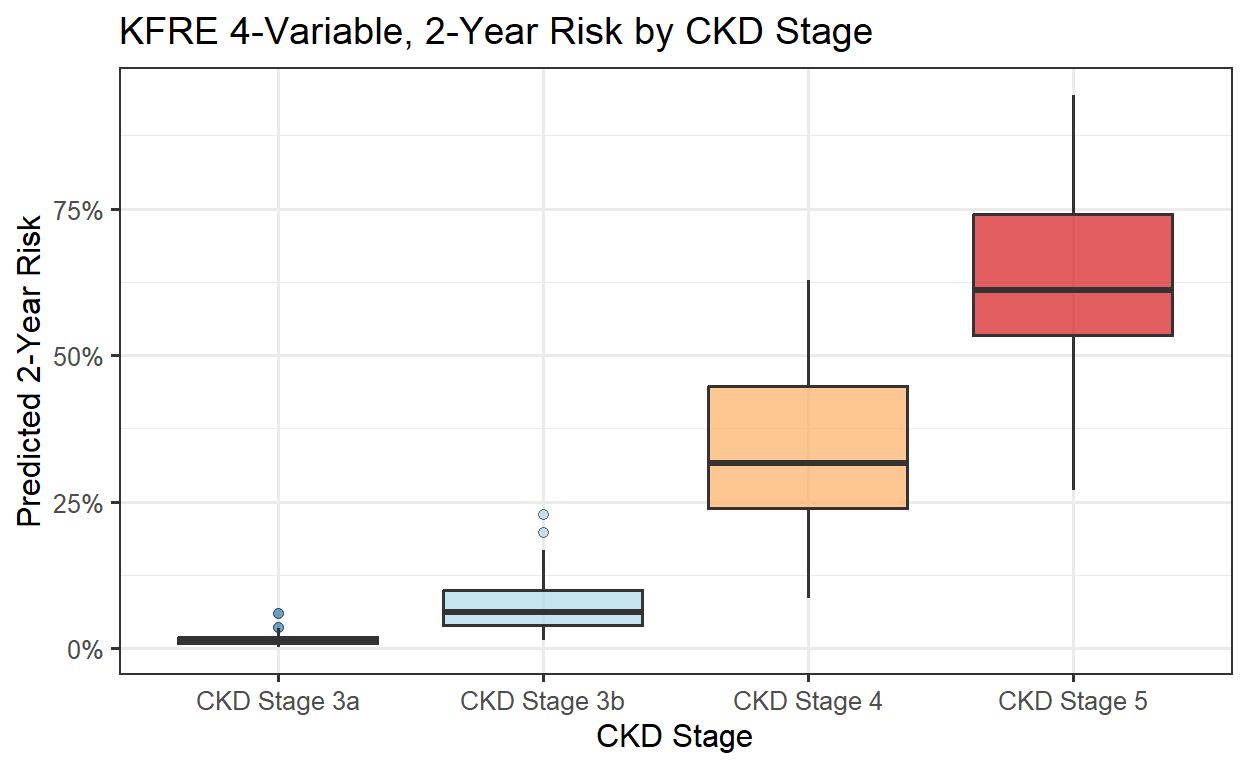
\includegraphics[width=0.9\linewidth]{kfre-paper_files/figure-latex/risk-by-stage-1.png} 

}

\caption{Distribution of 4-variable, 2-year KFRE predicted risk by CKD stage in synthetic cohort.}\label{fig:risk-by-stage}
\end{figure}

\subsection{Comparing model variants}\label{comparing-model-variants}

\begin{figure}

{\centering 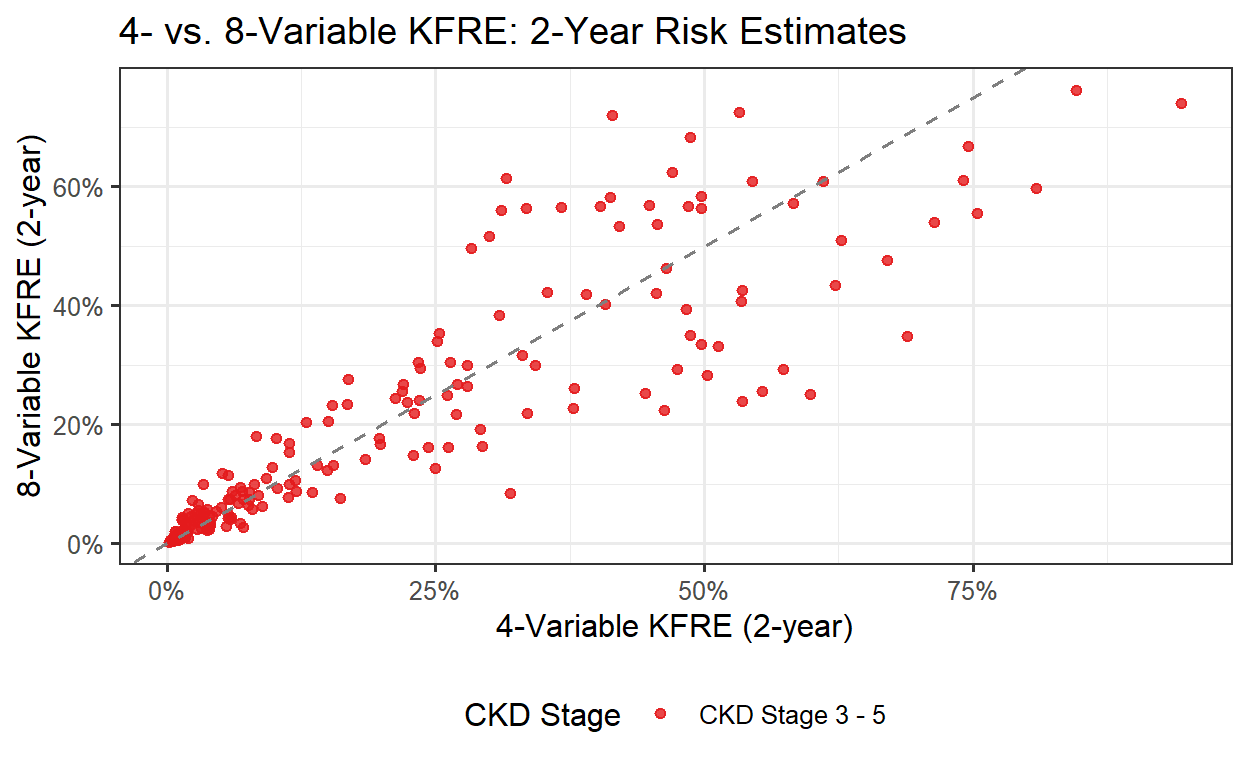
\includegraphics[width=0.9\linewidth]{kfre-paper_files/figure-latex/model-comparison-1.png} 

}

\caption{Predicted 2-year risk: 4-variable vs. 8-variable KFRE in synthetic cohort.}\label{fig:model-comparison}
\end{figure}

The 4- and 8-variable models produce closely correlated estimates
(Figure \ref{fig:model-comparison}), with systematic divergence at higher risk
levels reflecting the additional information contributed by the extended
laboratory variables.

\section{Discussion}\label{discussion}

\textbf{kfre} provides the R community with a comprehensive, tested, and
reproducible implementation of the Kidney Failure Risk Equation. The package
addresses a practical gap: the KFRE is now a guideline-recommended clinical
tool used globally, yet analysts working in R were previously required to
implement the equations manually or adapt code from other sources. \textbf{kfre}
consolidates the full analytical workflow from raw data processing through risk
prediction, staging, evaluation, and visualization into a single, cohesive
package.

Several design decisions merit explicit discussion. First, the three-interface
architecture (functional, data-frame wrapper, R6) is unusual but deliberate. A
single-function approach would have forced trade-offs between ease of use for
interactive work and ergonomics for pipeline development; the three interfaces
address these use cases without duplicating logic. Second, the naming convention
for output columns (\texttt{kfre\_\{n\}var\_\{t\}year}) is enforced consistently across
\texttt{add\_kfre\_risk\_col()}, \texttt{eval\_kfre\_metrics()}, and \texttt{plot\_kfre\_metrics()}, so
that the output of one function can be passed directly to the next without
renaming.

\textbf{Limitations.} The KFRE coefficients implemented in \textbf{kfre} are those
published by \citet{tangri2011} and \citet{tangri2016}. Recent work, including the 59-cohort
CKD Prognosis Consortium study using the 2021 CKD-EPI creatinine equation
\citep{grams2023}, has evaluated the KFRE with updated eGFR-estimating equations and
found generally good performance for eGFR \textless{} 45 mL/min/1.73 m\(^2\). Users
applying \textbf{kfre} in populations with eGFR between 45 and 60, or in settings
where competing risks from all-cause mortality are substantial, should consult
this literature before interpreting predictions. Second, the non-North American
calibration factor shifts the baseline survival probability for non-North
American cohorts, but users should verify calibration in their own population
before clinical deployment. Third, the uPCR-to-uACR conversion from \citet{sumida2020}
introduces its own measurement uncertainty; direct uACR measurement remains
preferable when available.

\textbf{Future directions.} Planned extensions include support for updated coefficient
sets as they are published, confidence interval estimation via bootstrapping, and
a Shiny-based interface for single-patient point-of-care use. Contributions and
bug reports are welcomed via the GitHub issue tracker at
\url{https://github.com/lshpaner/kfre_r/issues}.

\textbf{kfre} is available on CRAN and is distributed under the MIT License.

\section*{Acknowledgments}\label{acknowledgments}
\addcontentsline{toc}{section}{Acknowledgments}

The author thanks the developers of the \textbf{R6}, \textbf{ggplot2}, \textbf{pROC},
and \textbf{precrec} packages on which \textbf{kfre} depends.


\bibliography{kfre}
\address{%
Leonid Shpaner\\
UCLA\\%
Los Angeles, CA\\
%
%
%
\href{mailto:lshpaner@ucla.edu}{\nolinkurl{lshpaner@ucla.edu}}%
}
